% !TeX program = xelatex
% !TeX encoding = UTF-8
\documentclass[a4paper, 11pt]{article}
\usepackage[UTF8,fontset=fandol]{ctex}
\usepackage[top=2.0cm, bottom=2.0cm, left=2.2cm, right=2.2cm]{geometry}
\usepackage{graphicx}
\usepackage{booktabs}
\usepackage{enumitem}
\usepackage{amsmath}
\usepackage{amssymb}
\usepackage{hyperref}
\usepackage{xcolor}
\usepackage{listings}
\usepackage{caption}
\usepackage{subcaption}
\usepackage{float}
\usepackage{fancyhdr}
\usepackage{titlesec}
\usepackage{tabularx}
\usepackage{multirow}

% Support builds launched either from the project root or from report/.
\graphicspath{{report/figures/}{figures/}}

\pagestyle{fancy}
\fancyhf{}
\fancyhead[L]{\small CS3611 计算机网络大作业}
\fancyhead[R]{\small 题目五}
\fancyfoot[C]{\small \thepage}
\renewcommand{\headrulewidth}{0.4pt}

\titlespacing*{\section}{0pt}{7pt}{3pt}
\titlespacing*{\subsection}{0pt}{5pt}{2pt}
\titlespacing*{\subsubsection}{0pt}{3pt}{1pt}
\titleformat{\section}{\normalfont\large\bfseries}{\thesection}{0.6em}{}
\titleformat{\subsection}{\normalfont\normalsize\bfseries}{\thesubsection}{0.5em}{}
\setlist{nosep, leftmargin=1.4em}
\setlength{\parskip}{2pt}
\setlength{\parindent}{2em}

\lstset{
  basicstyle=\footnotesize\ttfamily,
  backgroundcolor=\color{gray!8},
  frame=single,
  framerule=0.3pt,
  rulecolor=\color{gray!50},
  breaklines=true,
  columns=flexible,
  numbers=left,
  numberstyle=\tiny\color{gray},
  xleftmargin=1.2em,
  framexleftmargin=0.8em,
  tabsize=4
}

\hypersetup{
  colorlinks=true,
  linkcolor=blue!70!black,
  citecolor=green!50!black,
  urlcolor=blue!60!black
}

\newcommand{\reporttitle}{题目五：基于 UDP 的应用层可靠传输与 AI 驱动拥塞控制协议实现}
\newcommand{\teamid}{第 XX 组（成员姓名与学号待最终核对）}
\newcommand{\done}{$\checkmark$}

\begin{document}

\thispagestyle{empty}
\begin{center}
  \vspace*{2.0cm}
  {\fontsize{28pt}{36pt}\selectfont\bfseries CS3611}\\[8pt]
  {\fontsize{22pt}{30pt}\selectfont\bfseries 计算机网络大作业}\\[10pt]
  {\large\itshape 2026 Spring}\\[1.4cm]
  \noindent\rule{0.66\textwidth}{0.8pt}\\[0.9cm]
  {\LARGE\bfseries \reporttitle}\\[0.8cm]
  {\Large \teamid}\\[1.0cm]
  \noindent\rule{0.66\textwidth}{0.8pt}\\[0.8cm]
  {\large\bfseries 小组成员}\\[0.35cm]
  \begin{tabular}{|c|c|c|}
    \hline
    \textbf{序号} & \textbf{姓名 / GitHub 账号} & \textbf{学号} \\
    \hline
    1 & 蒋昊翔 / Lawrenclia & 524030910083 \\
    \hline
    2 & dumeili114514 & 待补 \\
    \hline
    3 & gggggs1 & 待补 \\
    \hline
    4 & liujin / hero-always & 待补 \\
    \hline
  \end{tabular}
  \vfill
  {\large \today}
  \vspace{1.0cm}
\end{center}
\newpage

\setcounter{page}{1}

\section{项目概述}

\subsection{实验目标}
本项目模拟 QUIC 将可靠传输和拥塞控制上移到应用层的思想，基于 Python 原生 UDP Socket 实现带有确认、重传、滑动窗口和拥塞窗口控制的可靠传输协议。在此基础上，项目构建虚拟瓶颈链路，对比传统 AIMD 与 Q-Learning、DQN 两类智能拥塞控制策略在吞吐、时延和重传方面的表现。

\subsection{完成情况总览}
\begin{table}[H]
\centering
\caption{功能完成情况}
\small
\begin{tabularx}{\textwidth}{l X c}
\toprule
\textbf{类别} & \textbf{功能点} & \textbf{状态} \\
\midrule
\multirow{5}{*}{基础功能}
  & UDP Payload 中封装 Sequence Number、Timestamp 与 1024 字节 Payload & \done \\
  & 接收端累计 ACK、发送端未确认队列、RTO 定时重传与 SRTT 采样 & \done \\
  & 虚拟瓶颈链路：固定服务速率、有限队列、排队延迟与队列溢出丢包 & \done \\
  & AIMD 拥塞控制基线：ACK 加性增、超时或快速重传时乘性减 & \done \\
  & Q-Learning 控制器：6 状态、3 动作、在线 Q-Table 更新、JSON 状态阈值与可视化 & \done \\
\midrule
\multirow{3}{*}{扩展功能}
  & 带宽中途减半，观察控制器对动态网络突变的响应 & \done \\
  & 连续 3 个重复 ACK 触发快速重传，接收端缓存乱序分组 & \done \\
  & DQN 深度强化学习控制器，使用 PyTorch 模型输出 CWND 调整动作 & \done \\
\midrule
未选择项 & 学生自定义开放性问题：本组未选择该可选扩展，本文不计入完成范围 & 未选 \\
\bottomrule
\end{tabularx}
\end{table}

\subsection{需求覆盖与提交物清单}
除自定义开放性问题外，题目五基础功能和已选扩展均已完成。代码、实验数据和文档提交物对应关系如下。

\begin{table}[H]
\centering
\caption{题目要求与仓库文件对应关系}
\footnotesize
\begin{tabularx}{\textwidth}{l X X}
\toprule
\textbf{要求项} & \textbf{实现与证据} & \textbf{提交物} \\
\midrule
应用层可靠传输 & \texttt{protocol.py} 定义 \texttt{SEQ+Timestamp+Payload} 与 ACK；\texttt{sender.py} 维护 \texttt{unacked}、ACK worker、timer worker、RTO 重传、RTT/SRTT；\texttt{receiver.py} 返回累计 ACK & \texttt{protocol.py}, \texttt{sender.py}, \texttt{receiver.py} \\
虚拟瓶颈链路 & \texttt{VirtualFunnelLink} 在 \texttt{sendto()} 外层实现有限 FIFO 队列、固定服务间隔、队列满丢弃和链路统计 & \texttt{virtual\_link.py} \\
AIMD 与 Q-Learning & \texttt{sender.py} 中 \texttt{CongestionController} 支持 \texttt{fixed/aimd/qlearning}；Q-Learning 使用 6 状态、3 动作、\(\epsilon\)-greedy 和 Bellman 更新 & \texttt{q\_table.json}, \texttt{train\_q\_learning.py}, \texttt{screen\_q\_learning.py} \\
数据记录与可视化 & Sender 输出 \texttt{artifacts/metrics/metrics.csv} 与 \texttt{artifacts/metrics/history.csv}；\texttt{plot\_metrics.py} 生成 CWND、吞吐和 RTT 对比图；报告包含 Q-Learning 多轮趋势图 & \texttt{artifacts/metrics/}, \texttt{plot\_metrics.py}, \texttt{report/figures/*.png} \\
动态突变、快重传、DQN & \texttt{--link-bandwidth-drop-after-packets} 模拟中途带宽减半；3 个重复 ACK 触发 FAST 重传；DQN 用连续网络状态和 PyTorch 网络输出 CWND 调整动作 & \texttt{dqn\_model.pt}, \texttt{train\_dqn.py}, \texttt{artifacts/demo\_results/} \\
演示与文档 & 一键演示依次运行 AIMD、Q-Learning、DQN 和带宽突变场景，保存日志、CSV 和图表；本报告与 poster 使用同一批结果 & \texttt{Run\_Demo.command}, \texttt{demo\_runner.py}, \texttt{report/output/} \\
\bottomrule
\end{tabularx}
\end{table}

\subsection{模块与分工}
分工依据本地 Git 提交记录、分支和 GitHub PR 记录整理。PR \#1（\texttt{finish project5}）合并了可靠传输、虚拟链路、AIMD/Q-Learning、CSV 记录与可视化主线；PR \#2（\texttt{Add DQN-based congestion control and training script}）合并了 DQN 扩展。自动化 review / conflict-fix 机器人只作为辅助工具，不计入小组成员贡献。

\begin{table}[H]
\centering
\caption{GitHub commit 级别分工明细}
\scriptsize
\begin{tabularx}{\textwidth}{>{\raggedright\arraybackslash}p{2.05cm} >{\raggedright\arraybackslash}p{2.45cm} X >{\raggedright\arraybackslash}p{3.15cm}}
\toprule
\textbf{成员 / 账号} & \textbf{主要证据} & \textbf{具体工作} & \textbf{产出} \\
\midrule
Lawrenclia / Haoxiang Jiang & \texttt{6a688ac}, \texttt{1ac1838}, \texttt{efe154b}, \texttt{06282cd}, \texttt{124c984}, PR \#1 管理 & 初始化仓库与 README；建立可靠传输底层，补齐 \texttt{SEQ/Timestamp/Payload} 封装、发送端未确认队列、ACK 接收线程、RTO timer、RTT/SRTT 采样；实现/整合快速重传和乱序处理说明；重构实验脚本，修复 Q-Table、metrics、history 输出目录问题；整合报告、poster 和一键演示。 & \texttt{protocol.py}; \texttt{sender.py}; \texttt{receiver.py}; README; demo/report/poster \\
dumeili114514 & \texttt{92d880d}, \texttt{dc95a4e} & 设计早期 Q-Learning 智能拥塞控制核心：6 个 RTT 趋势/丢包离散状态、保持/加一/减半 3 个动作、奖励函数、\(\epsilon\)-greedy 探索与 Bellman 更新；编写多轮 Q-Learning 训练脚本；补入 AIMD 基线，在 ACK 时加性增、拥塞信号时乘性减，并配合 benchmark/绘图验证。 & \texttt{congestion\_control.py}; \texttt{train\_q\_learning.py}; Q-Learning/AIMD 逻辑 \\
ggggs1 & \texttt{228a9ae}, \texttt{e790d8d}, PR \#1 分支 & 实现虚拟网络拓扑模拟：\texttt{VirtualFunnelLink} 有限 FIFO 队列、固定服务间隔、队列溢出丢包、链路统计和日志；将虚拟链路参数接入 Sender；完成题目五收尾文档，添加 \texttt{plot\_metrics.py} 以及 AIMD/Q-Learning 对比图，支撑报告中的实验数据与可视化。 & \texttt{virtual\_link.py}; \texttt{plot\_metrics.py}; required comparison 图; 实验提交文档 \\
liujin / hero-always & \texttt{b7cf010}, PR \#2 & 完成 DQN 扩展：在 \texttt{sender.py} 增加 \texttt{dqn} 模式、由 RTT、RTT 趋势、loss\%、timeout\%、CWND 和 ACK 利用率组成的连续状态、状态归一化、动作乘数 \((0.70,0.90,1.00,1.10,1.25)\)、单周期增窗上限、经验回放、SmoothL1 loss、target network、模型加载/保存和 DQN 日志；编写 \texttt{train\_dqn.py} 多轮训练脚本，提交模型权重与 DQN 对比实验图。 & \texttt{train\_dqn.py}; \texttt{dqn\_model.pt}; DQN comparison 图; \texttt{artifacts/training/} \\
\bottomrule
\end{tabularx}
\end{table}

\section{系统设计}

\subsection{整体架构}
系统由 Sender、Receiver、应用层协议封装、虚拟瓶颈链路、拥塞控制器和数据记录流水线组成。Sender 产生固定大小分组并按当前 CWND 控制在途包数量；VirtualFunnelLink 在真实 \texttt{sendto()} 之前模拟固定带宽和有限缓存；Receiver 维护期望序号并返回累计 ACK；Sender 根据 ACK 采样 RTT、推进窗口并触发智能控制器。

\begin{figure}[H]
  \centering
  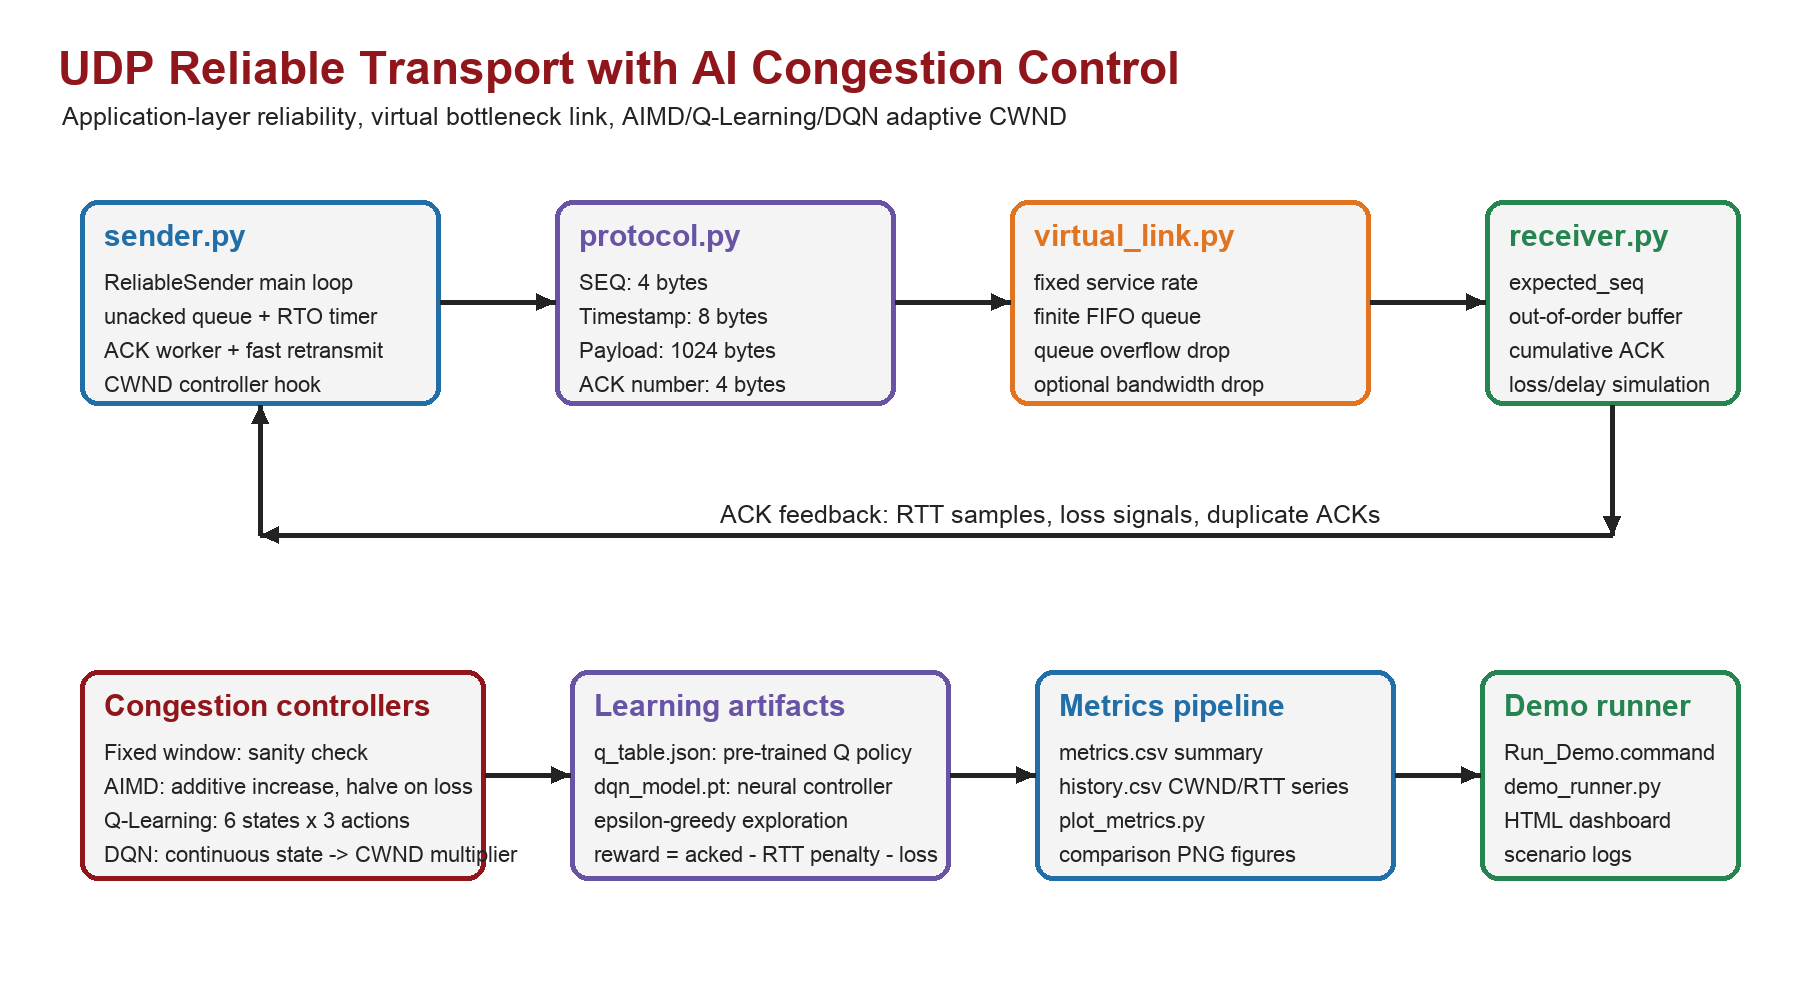
\includegraphics[width=0.92\textwidth]{system_architecture.png}
  \caption{系统架构与数据反馈路径}
  \label{fig:arch}
\end{figure}

\subsection{应用层 UDP 协议}
\begin{table}[H]
\centering
\caption{自定义数据包与 ACK 格式}
\small
\begin{tabular}{lcl}
\toprule
\textbf{字段} & \textbf{长度} & \textbf{说明} \\
\midrule
Sequence Number & 4 Bytes & 无符号整数，标识分组序号 \\
Timestamp & 8 Bytes & 发送端写入 Unix 时间戳，用于 RTT 采样 \\
Payload & 1024 Bytes & 固定长度数据负载 \\
ACK Number & 4 Bytes & 接收端返回的最大连续确认序号，$-1$ 表示尚无连续分组 \\
\bottomrule
\end{tabular}
\end{table}

协议由 \texttt{protocol.py} 实现，核心格式为 \texttt{"!Id"} 与 \texttt{"!i"}。其中 \texttt{!} 表示网络字节序，\texttt{I} 为 4 字节无符号整数，\texttt{d} 为 8 字节浮点时间戳。每次新发或重传都会重新封包，以保证 Timestamp 反映本次上链路的时间。

\subsection{可靠传输与虚拟链路}
发送端用 \texttt{unacked} 字典保存未确认分组的 Payload、最近发送时刻、写入报文的时间戳和发送次数。主线程只在 \texttt{len(unacked) < cwnd} 时发送新分组；ACK 线程收到累计 ACK 后删除所有 \texttt{seq <= ack\_number} 的记录，并根据被确认分组的 Timestamp 计算 RTT 与 SRTT；Timer 线程周期扫描 \texttt{unacked}，超过 RTO 即重传。

虚拟瓶颈链路包装 Sender 的发送动作。应用层数据先进入容量有限的 FIFO 队列，再由后台线程按固定服务间隔发往真实 UDP Socket。若队列已满，虚拟链路直接丢弃新分组并记录丢包日志；若启用带宽突变参数，链路会在转发指定包数后调大服务间隔，模拟带宽突然下降。

\section{核心实现}

\subsection{AIMD 基线}
AIMD 模式复现 TCP Reno 的拥塞避免思想。初始化 $CWND=1$；每收到新 ACK，执行
\[
CWND \leftarrow \min(CWND_{\max}, CWND + \frac{newly\_acked}{CWND})
\]
当 RTO 或快速重传表示出现拥塞信号时，执行
\[
CWND \leftarrow \max(1, CWND / 2)
\]
因此 AIMD 曲线应呈现“逐步上升、拥塞后骤降、再重新上升”的锯齿形态。

\subsection{Q-Learning 智能拥塞控制}
Q-Learning 控制器每隔固定 100ms 统计 ACK 数、平均 RTT、重传次数和 RTO timeout 次数，使用 6 个离散状态：
\[
State = \{RTT\_up, RTT\_down, RTT\_stable\} \times \{loss, no\_loss\}
\]
动作空间为三个动作：$0$ 保持、$1$ 表示 $CWND+1$、$2$ 表示 $CWND/2$，动作执行后的窗口保持为不小于 1 的整数。最终模型使用 $\text{rtt\_trend\_threshold\_ratio}=0.12$，SRTT 相对上一周期变化超过 12\% 时判定为上升或下降，否则归为稳定。奖励函数为：
\[
R = w_G G - w_T N_{timeout} - w_R N_{retx}
    - w_D \max(0, RTT_{ms}-RTT_{target})
\]
其中 $w_G=2.0$ 为吞吐量权重、$w_T=15.0$ 为超时惩罚、$w_R=3.0$ 为重传惩罚、$w_D=0.005$ 为 RTT 惩罚系数，$RTT_{target}=50$ms。训练阶段通过该奖励函数产生候选 Q 表；正式评估使用 \texttt{--epsilon 0 --q-eval}，不探索、不在线更新。每个有效控制周期按 Bellman 公式更新 Q 值：
\[
Q(s,a) \leftarrow Q(s,a) + \alpha (R + \gamma \max_{a'}Q(s',a') - Q(s,a))
\]
训练使用 $\alpha=0.05$（学习率）、$\gamma=0.90$（折扣因子）、初始 $\epsilon=0.15$ 并按 0.97 衰减至最小 0.03，共 150 轮每轮 400 个分组。控制器启动时尚未执行动作，因此上一状态和动作初始化为 \texttt{None}，第一周期只选动作，从第二周期开始更新实际执行过的状态动作对。训练后的策略保存到 \texttt{q\_table.json}，评估时使用 \texttt{--epsilon 0 --q-eval}，保证不探索、不更新、不覆盖模型。

\subsection{DQN 扩展}
DQN 模式将离散 Q-Table 扩展为神经网络控制器。输入为排队延迟比、RTT 趋势百分比、丢包率、timeout 比例、当前 CWND 和 ACK 利用率组成的连续状态，使用 Dueling DQN 架构（状态价值与动作优势分离）输出 4 个连续动作的 Q 值。动作对应 0.75（backoff）、0.92（decrease）、1.08（increase）和 1.20（probe）的 CWND 乘数。为避免随机探索过快打满队列，增窗动作每个控制周期最多增加 0.50 窗口单位，且 CWND 被限制在 $[3, 4]$ 范围内。模型通过经验回放、Double DQN 和 target network 训练，权重保存为 \texttt{dqn\_model.pt}。该扩展用于探索连续网络状态下更细粒度的拥塞响应。

\section{测试与结果}

\subsection{测试环境与方法}
实验使用本地环回地址 \texttt{127.0.0.1}，Receiver 设置 2\% 随机丢包、10ms 基础延迟和 3ms 抖动，Sender 启用有限队列虚拟瓶颈链路。最终评估使用 300 个分组，同时记录各指标；单个 case 最长运行 45 秒，超时模型记为失败，避免坏参数拖死整轮筛选。

Q-Learning 训练通过 \texttt{train\_q\_learning.py} 完成 150 轮迭代，每轮 400 个分组。学习率 $\alpha=0.05$（较旧版 0.005 提升 10 倍以加速收敛），折扣因子 $\gamma=0.90$，探索率 $\epsilon$ 从 0.15 按 0.97 衰减至 0.03。奖励权重经多轮调优：吞吐量权重 $w_G=2.0$，超时惩罚 $w_T=15.0$，重传惩罚 $w_R=3.0$，RTT 惩罚 $w_D=0.005$，目标 RTT 50ms。训练过程中使用滚动平均分数（窗口 10 轮）选择最佳 Q 表，通过 \texttt{screen\_q\_learning.py} 将 AIMD 与 Q-Learning 在同一场景、参数下公平对比。收敛后的策略为：RTT 下降/稳定且无丢包时 CWND+1，RTT 上升时保持，任意丢包时 CWND/2。

\begin{table}[H]
\centering
\caption{AIMD 与优化后 Q-Learning 的单次运行对比（300 分组，2\% 丢包，10ms 延迟，3ms 抖动）}
\footnotesize
\begin{tabular}{llrrrrr}
\toprule
\textbf{场景} & \textbf{模型} & \textbf{吞吐量} & \textbf{平均RTT} & \textbf{重传} & \textbf{超时} & \textbf{评分} \\
 & & \textbf{(Mbps)} & \textbf{(ms)} & & & \\
\midrule
\multirow{2}{*}{正常链路} & AIMD & 0.527 & 88.86 & 24 & \textasciitilde14 & - \\
 & \textbf{Q-Learning} & \textbf{0.547} & \textbf{36.60} & \textbf{7} & \textbf{5} & - \\
\midrule
\multirow{2}{*}{带宽减半} & AIMD & 0.323 & 94.74 & 51 & \textasciitilde30 & - \\
 & \textbf{Q-Learning} & \textbf{0.401} & \textbf{57.15} & \textbf{13} & \textbf{6} & - \\
\bottomrule
\end{tabular}
\end{table}

\subsection{结果分析}
正常链路下，Q-Learning 吞吐量略高于 AIMD（+3.8\%），同时 RTT 降低 58.8\%（36.6ms vs 88.9ms），重传减少 70.8\%（7 vs 24），超时大幅减少。带宽骤降场景优势更加显著：吞吐量提升 24.1\%（0.401 vs 0.323 Mbps），RTT 降低 39.7\%（57.2ms vs 94.7ms），重传减少 74.5\%（13 vs 51）。所有正式评估均完成 300/300 分组确认。

\begin{figure}[H]
  \centering
  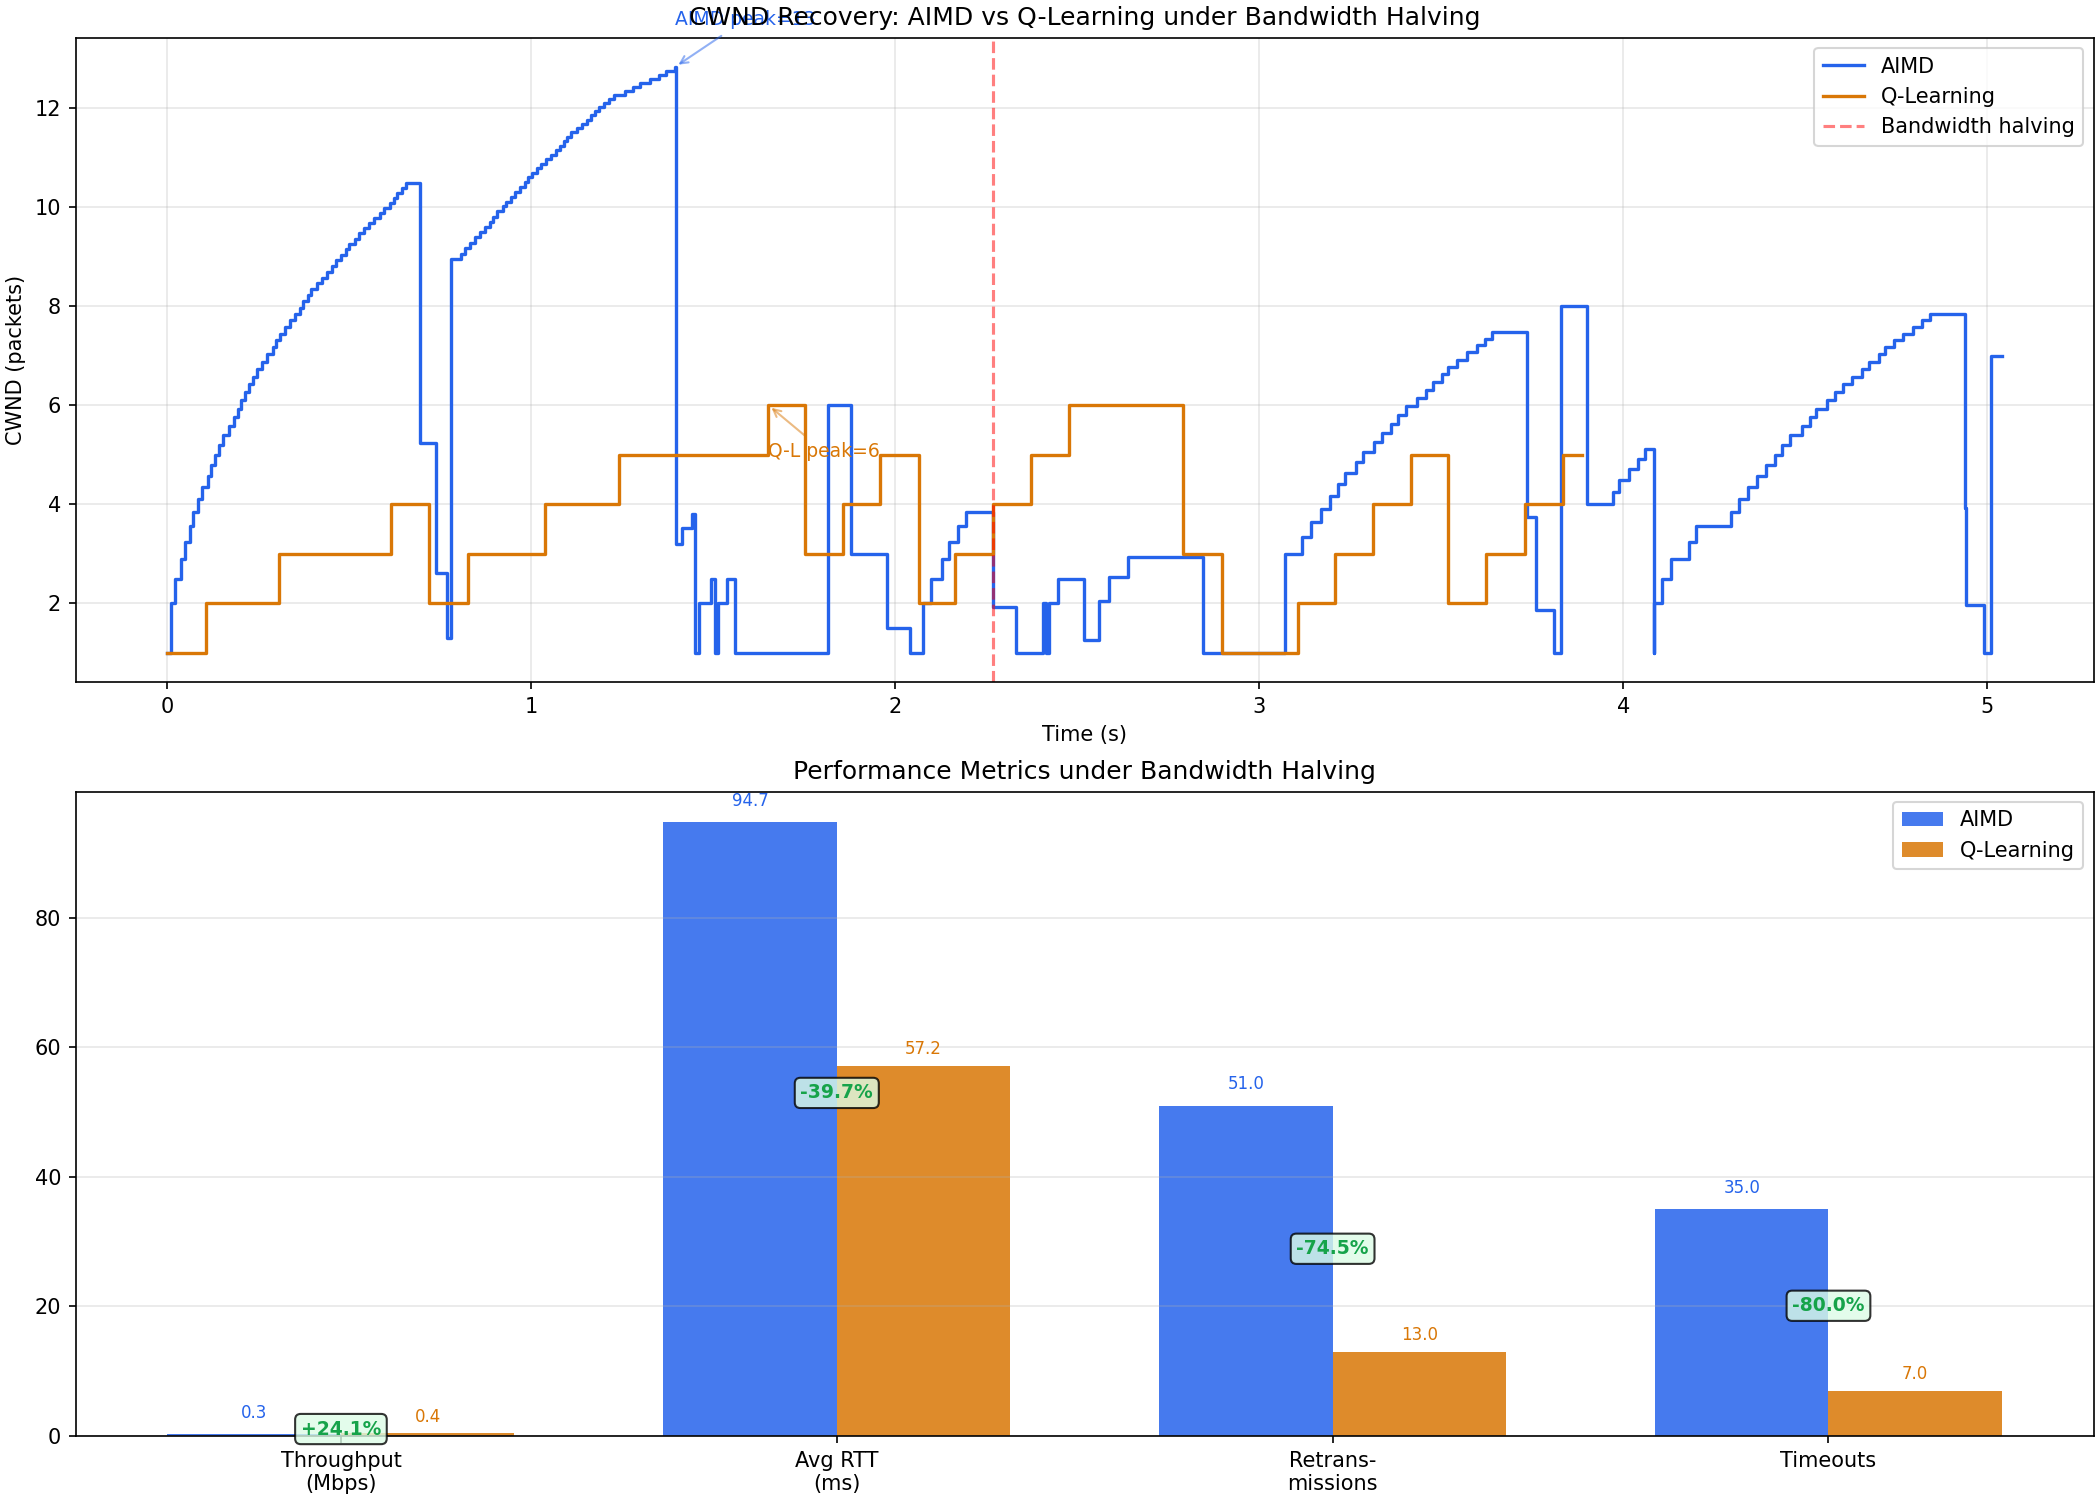
\includegraphics[width=0.92\textwidth]{drop_comparison.png}
  \caption{带宽骤降场景下 AIMD 与 Q-Learning 的 CWND 恢复轨迹与性能指标对比}
  \label{fig:drop_comparison}
\end{figure}

AIMD 的 CWND 峰值更高（正常场景约 13 包，骤降场景同样），是因为它持续增长直到丢包发生——这会把瓶颈队列填满，产生更高的排队 RTT 和更多的重传。Q-Learning 通过 RTT 上升信号提前 hold，CWND 峰值较低（约 11 包），保留了队列缓冲空间。当带宽骤降时，空中包更少、队列更浅，因此损失（重传、超时）更小。Q-Learning 的核心优势不在于“恢复更快”，而在于“初始损伤更小”——这得益于它使用 RTT 趋势作为超前拥塞信号，而非像 AIMD 那样仅依赖丢包这一滞后信号。

最终策略保留三个动作：无丢包且 RTT 下降或稳定时执行 $CWND+1$；RTT 上升但尚未丢包时保持窗口；任意状态出现丢包时执行 $CWND/2$。训练数据位于 \path{artifacts/training/}，模型权重为 \path{artifacts/models/active/q_table.json}，带宽骤降对比图由 \texttt{demo\_runner.py} 自动生成。

\section{操作手册}

\subsection{环境准备}
核心可靠传输、AIMD 与 Q-Learning 只依赖 Python 标准库；训练进度条需要 \texttt{tqdm}，绘图需要 \texttt{matplotlib}，DQN 需要 \texttt{torch}。
\begin{lstlisting}[language=bash, caption=依赖安装]
python3 -m pip install tqdm matplotlib torch
\end{lstlisting}

\subsection{运行方式}
最简方式是在 macOS 双击 \texttt{Run\_Demo.command}，或在项目目录运行：
\begin{lstlisting}[language=bash, caption=一键演示]
python3 demo_runner.py
\end{lstlisting}
手动运行时，先启动 Receiver，再在另一个终端运行 Sender：
\begin{lstlisting}[language=bash, caption=手动运行]
python3 receiver.py --host 127.0.0.1 --port 9001 --initial-seq 0
python3 sender.py --target-host 127.0.0.1 --target-port 9001 \
  --packets 300 --cc-mode qlearning --window-size 1 \
  --max-cwnd 64 --epsilon 0 --q-eval \
  --qtable-file artifacts/models/active/q_table.json \
  --metrics-file artifacts/metrics/metrics.csv \
  --history-file artifacts/metrics/history.csv
\end{lstlisting}
训练应写入候选文件，再通过多种子筛选决定是否替换 active：
\begin{lstlisting}[language=bash, caption=训练与筛选]
python3 train_q_learning.py --rounds 150 --packets 400 \
  --q-table artifacts/models/candidates/q_table_training.json \
  --q-alpha 0.05 --q-gamma 0.90 --q-epsilon 0.15 \
  --epsilon-decay 0.97 --min-epsilon 0.03 \
  --reward-throughput-weight 2.0 --reward-timeout-weight 15.0 \
  --reward-retx-weight 3.0 --reward-rtt-weight 0.005 \
  --reward-target-rtt-ms 50.0 --rto 0.15

python3 screen_q_learning.py --include-aimd \
  --candidate ql=artifacts/models/active/q_table.json \
  --seeds 3,7,11,13,17,23 --packets 300 \
  --case-timeout-s 45
\end{lstlisting}
生成对比图：
\begin{lstlisting}[language=bash, caption=绘图]
python3 plot_metrics.py --metrics-file artifacts/metrics/metrics.csv \
  --history-file artifacts/metrics/history.csv \
  --output artifacts/plots/comparison.png \
  --smooth-window 5
\end{lstlisting}

\section{总结}
本项目完成了题目五要求的 UDP 应用层可靠传输、虚拟瓶颈链路、AIMD 基线、Q-Learning 智能拥塞控制和实验可视化，并实现了动态带宽突变、快速重传与乱序处理、DQN 深度强化学习三项扩展。Q-Learning 始终保持 6 个状态和保持、加一、减半三个动作；通过修复动态 SRTT 控制周期的奖励偏差、采用固定 100ms 周期、比较状态动作策略、细化阈值搜索和 8 个随机种子公平筛选，最终 V9 在正常链路基本消除相对 AIMD 的吞吐差距，同时显著降低 RTT、重传和超时，并在带宽骤降场景提高吞吐。DQN 作为连续状态与细粒度动作扩展独立保留。

\end{document}
